\documentclass[main.tex]{subfiles}
\begin{document}


\chapter{NEMO detectors}


%\begin{flushright}
%\textit{On peut braver les lois humaines, \\
%mais non résister aux lois naturelles}\\
%Jules Verne, \textit{Vingt mille lieues sous les mers.}
%\end{flushright} 


\NI Initiated in the late 1980s, the principal goals of the NEMO project are the search for 0$\nu\beta\beta$ decay and the measurement of 2$\nu\beta\beta$ decays. The strategy adopted by the collaboration is the direct detection of the two emitted electrons, by separating the $\beta\beta$ emitters from the rest of the detector. The Modane Underground Laboratory (LSM) have hosted all the NEMO prototypes and detectors. The LSM is shortly described in Section~\ref{sec:LSM}. Section~\ref{sec:NEMO3} and \ref{sec:SuperNEMO} present respectively NEMO-3 and SuperNEMO.


\section{Modane underground laboratory}\label{sec:LSM}


\NI Inaugurated in 1982, the Modane Underground Laboratory (LSM : Laboratoire Souterrain de Modane in french) is located in the Frejus tunnel at the border between France and Italy (Figure~\ref{LSMtunnel}).


\bigskip


\begin{figure}[h!]
\begin{center}
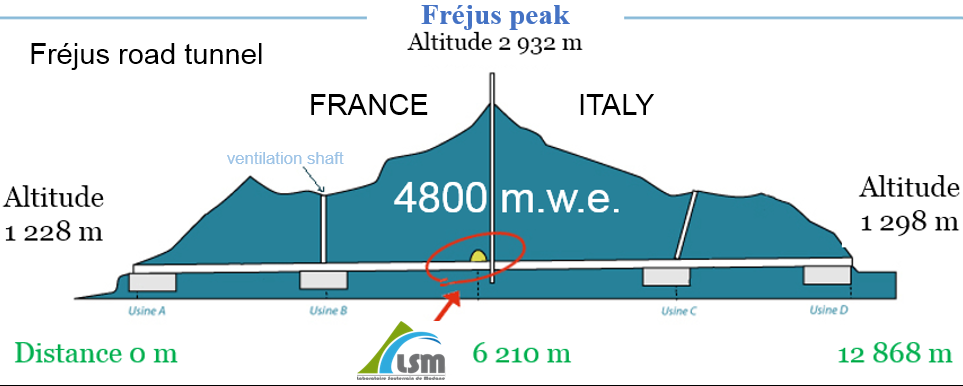
\includegraphics[scale=0.50]{pictures/Chap3/LSMtunnel.png}
\caption{Schematic view of the Modane underground laboratory location in the Frejus tunnel.}
\label{LSMtunnel}
\end{center}
\end{figure}

\NI The laboratory is sheltered from cosmic rays under 1700~meters of rocks (4200 meter water equivalent) which makes it the deepest underground laboratory in Europe and the third one in the world. The cosmic ray flux inside the laboratory have been measured to be 4/m$^\text{2}$/day [ref], compared to the million of particles arriving per m$^\text{2}$ at the surface of the Earth. The total muon flux for different underground laboratory is presented in~Figure~\ref{LabDeepth}.
 

\begin{figure}[h!]
\begin{center}
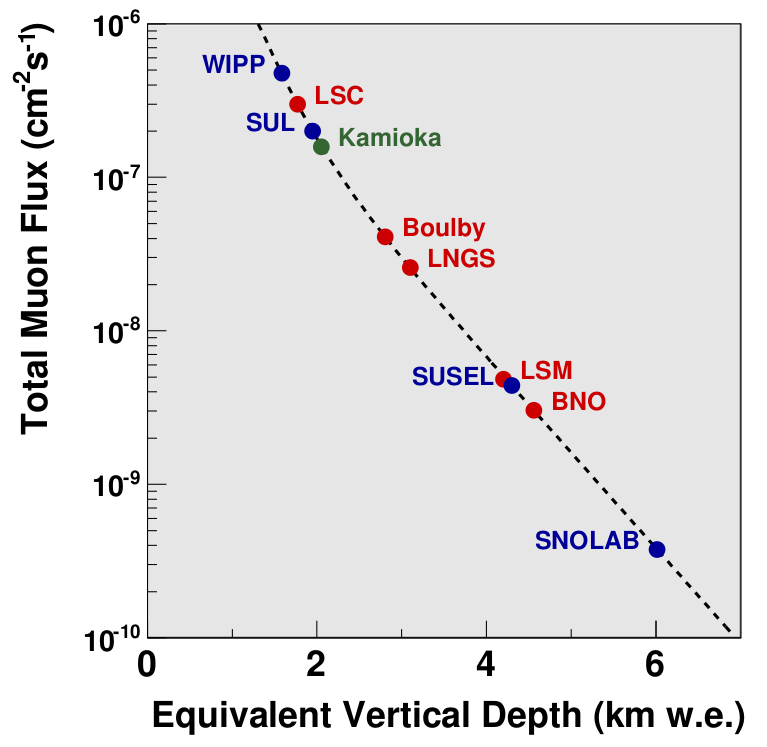
\includegraphics[scale=0.30]{pictures/Chap3/lab_depth.png}
\caption{Total muon flux in cm$^{\text{-2}}$.s$^{\text{-1}}$ with respect to the depth for different underground laboratory.}
\label{LabDeepth}
\end{center}
\end{figure}


\NI The protected environment of the laboratory is very favorable to the searches requiring very low backgrounds. Initially, the laboratory hosted an experiment searching for the proton decay. Latest, the laboratory diversified its activities, including astrophysics, biology, geology, electronics and environmental researches. The laboratory also have several High Purity Germanium detectors (HPGe) to measure very low radioactivity. 


\bigskip


\NI The two first NEMO prototypes were installed at LSM. They demonstrated that the reconstruction of low energy electrons was possible with the tracking system developed by NEMO [ref]. They also validated the strategy to measure background via different channels~[ref]. Then the laboratory hosted NEMO-3 during the 2000s. Today NEMO-3 have been replaced by SuperNEMO demonstrator which is currently under construction and commissionning phase.


\FloatBarrier


\section{NEMO-3}\label{sec:NEMO3}


\NI The NEMO-3 detector ran from February 2003 to January 2011 and searched for $\beta\beta$ decays among seven different isotopes. NEMO-3, shown in Figure~\ref{NEMO3Detector}, was a cylinder of 5~m in diameter and 3~m high. The detector was divided into 20 identical parts referred to as sectors. A picture of one of this sector is presented in Figure~\ref{NEMO3SectorPictures}. For the direct detection of two electrons, thin foils of $\beta\beta$ emitters were verticaly disposed at a fixed radius, as shown in Figure~\ref{TopViewNEMO3}. Placed on each side of the source foils, wire tracking chambers were used to measure the trajectory of charged particles. The tracker was allied to a magnetic field of 25~Gauss for charge identification. A calorimeter surrounded the tracking volume on all sides to provide both energy and timing measurements of particles. Passive shieldings of iron, paraffin, borated water and wood have been installed around the detector against cosmic rays and neutron interactions.


\begin{figure}[h!]
\begin{center}
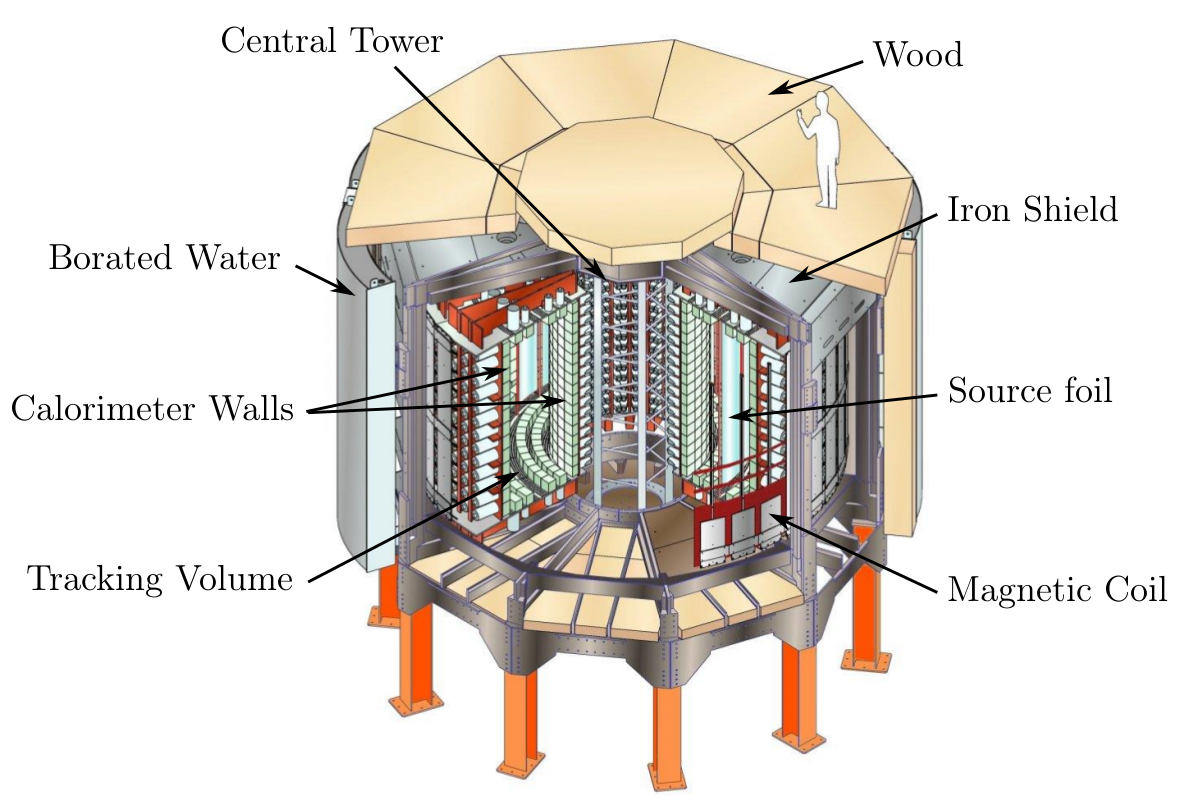
\includegraphics[scale=0.35]{pictures/Chap2/NEMO-3-Schema.png}
\caption{Exploded schematic view of the NEMO-3 detector.}
\label{NEMO3Detector}
\end{center}
\end{figure}


\NI This section provides an overview of each detector components based on the technical design report of NEMO-3 [ref]. Their calibrations and performances are also presented.  




\begin{figure}[h!]
\begin{center}
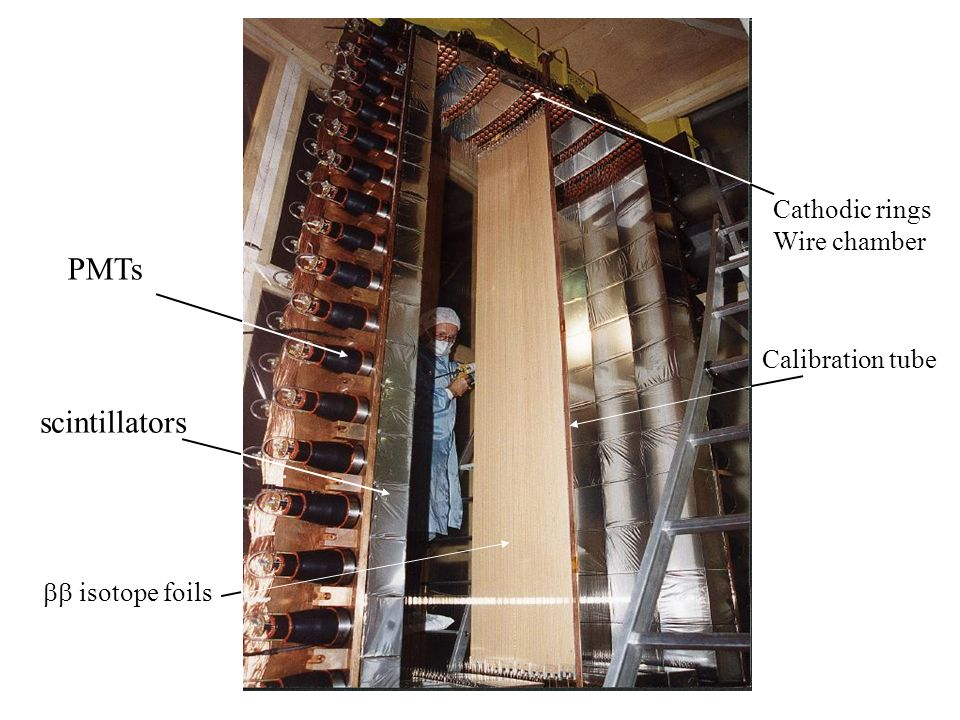
\includegraphics[scale=0.55]{pictures/Chap2/sector.jpg}
\caption{Picture of a NEMO-3 sector. A source foil is verticaly placed at the center and surrounded by a wire chamber. The tracker is enclosed by a calorimeter.}
\label{NEMO3SectorPictures}
\end{center}
\end{figure}


\begin{figure}[h!]
\begin{center}
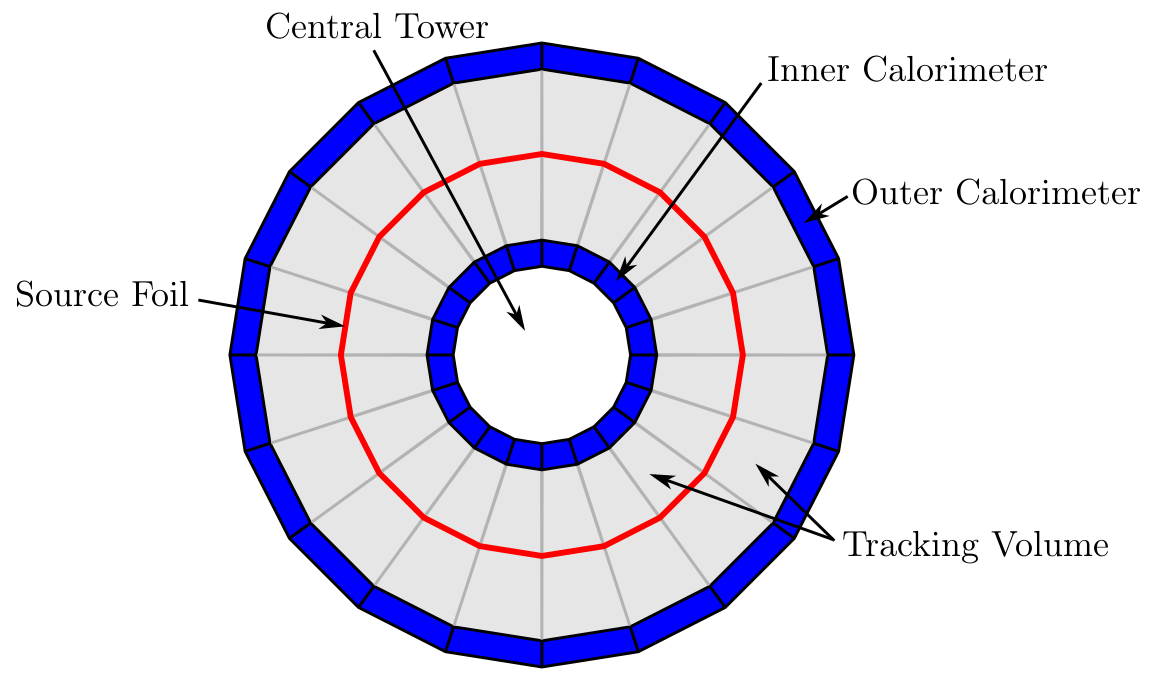
\includegraphics[scale=0.25]{pictures/Chap2/TopViewNEMO3.png}
\caption{Top view of the~NEMO-3~detector geometry. The cylinder is divided into 20 sectors, each containing source foil (red), tracker (grey) and calorimeter (blue).}
\label{TopViewNEMO3}
\end{center}
\end{figure}


\FloatBarrier


\subsection{Source foils}


\NI The separation of the source foils from the rest of the detector allows the investigation of any $\beta\beta$ emitters. A total of 8.8~kg of seven enriched isotopes have been introduced in the detector. The isotopes with the largest mass were $^{\text{100}}$Mo with 6.91~kg and $^{\text{82}}$Se with 0.93~kg. These two isotopes provide the best sensitivity to search for 0$\nu\beta\beta$ decays. Smaller quantities of five additionnal isotopes are included to measure the 2$\nu\beta\beta$ decay rate, including 0.45~kg of $^{\text{130}}$Te, 0.40~kg of $^{\text{116}}$Cd, 36.6~g of $^{\text{150}}$Nd, 9.43~g of $^{\text{96}}$Zr, and 6.99~g of $^{\text{48}}$Ca. The search for 0$\nu\beta\beta$ decay have also been performed with these isotopes. Alongside the enriched foils, 0.6~kg of very pure natural tellurium and 0.6~kg of ultra-pure copper foils were installed to control and validate the background measurements. The distribution of the isotopes around the 20 sectors are shown in Figure~\ref{NEMO3Sector}. The masses, Q$_{\beta\beta}$ values, half-lives and natural abundances for each of these $\beta\beta$ isotopes are given in Table~\ref{tab:isotopeNEMO3}.



\begin{figure}[h!]
\begin{center}
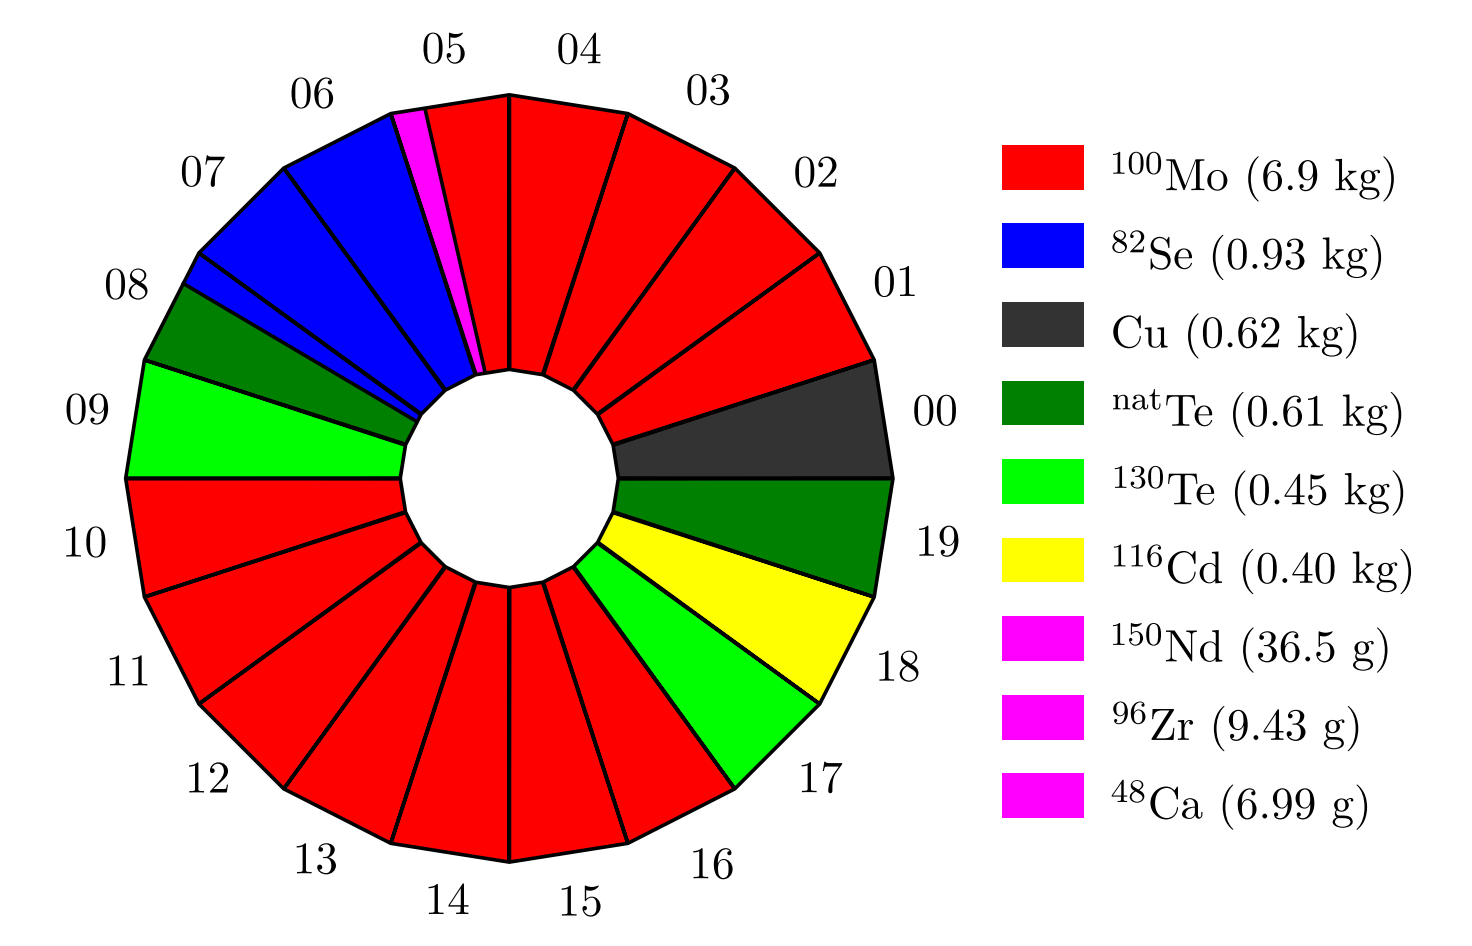
\includegraphics[scale=0.45]{pictures/Chap3/BBSourceDistribution.png}
\caption{Schematic view of the seven different $\beta\beta$ sources location inside the NEMO-3 detector. The main isotopes was $^{\text{100}}$Mo (6.9~kg) and $^{\text{82}}$Se (0.9~kg).}
\label{NEMO3Sector}
\end{center}
\end{figure}



\NI Each sector supports a source frame where seven strips of $\beta\beta$ emitter were placed. The five central strips were 2.48~m long and 6.5~cm wide, while the two border strips measured 2.48~m long and 6.3~cm wide. The thickness of the strips are in the range 30~-~60~mg/cm$^\text{2}$, which is a compromise to maximise the isotope mass while mainting the foil thin enough to reduce the scatterings through the foil bulk, and do not degrade the energy resolution.


\bigskip


\NI Two different kinds of foil were in NEMO-3, metallic and composite foils. The metallic foils (cadmium, molybdenum and copper) had a density of approximately 10~g/cm$^\text{3}$, which corresponds to a thickness a 60~$\mu$m. The composite foils (selenium, tellurium, zirconium, neodynium and calcium) are a mixture of source powder and organic glue. The density of the composite foil were approximately five times lower than the metallic foils, allowing to thickness up to 300~$\mu$s. The composite foils were surrounded by two mylar films to provide a mechanical strengh. To ensure a good bond with the glue and facilitate evaporation, the mylar sheets have a large number of microscopic holes.



\begin{table}[h!]
\centering
\begin{tabular}{c|c|c|c|c}
Isotopes & Mass [g] & Q$_{\beta\beta}$ [MeV] & T$_{\text{1/2}}^{\text{2}\nu}$ [y] & Abundance [\%]\\[0.05cm]
\toprule
$^{\text{100}}$Mo & 6 914 & 3.034 & 7.2 $\times$ 10$^{\text{18}}$ & 9.63 \\[0.1cm]
$^{\text{82}}$Se  & 932   & 2.995 & 9.6 $\times$ 10$^{\text{19}}$ & 8.73 \\[0.1cm]
$^{\text{130}}$Te & 454   & 2.529 & 7.0 $\times$ 10$^{\text{20}}$ & 33.8 \\[0.1cm]
$^{\text{116}}$Cd & 410 $\pm$ 1   & 2.802 & 2.9 $\times$ 10$^{\text{19}}$ & 7.49 \\[0.1cm]
$^{\text{150}}$Nd & 37    & 3.367 & 9.1 $\times$ 10$^{\text{18}}$ & 5.6  \\[0.1cm]
$^{\text{96}}$Zr  & 9.4   & 3.350 & 2.4 $\times$ 10$^{\text{19}}$ & 2.8  \\[0.1cm]
$^{\text{48}}$Ca  & 6.99  & 4.271 & 4.4 $\times$ 10$^{\text{19}}$ & 0.19 \\[0.1cm]
\bottomrule
\end{tabular}
\caption{Mass, Q$_{\beta\beta}$, T$_{\text{1/2}}^{\text{2}\nu}$ and abundance of the different isotopes introduced in NEMO-3.}
\label{tab:isotopeNEMO3}
\end{table} 


\subsection{The \texorpdfstring{\Cd}~ source foil}
\label{sec:CdSectorInNEMO3}


\NI A total mass of 440~g of cadmium were placed in sector 18. The average enrichment of \Cd~was (93.2~$\pm$~0.2)\%~\cite{NEMO-3-detector} which represents an effective mass of (410~$\pm$~1)~g~of~\Cd. The enrichment have been realized by the centrifugation separation method. Despite the good yield of this technique, smaller amounts of other cadmium isotopes are still present in the sample, see Table~\ref{IsotopeCdTable}. Part of the sample (152~g) was previously measured with the NEMO-2 prototype~\cite{ObservationCd116NEMO-2}.  


\bigskip


\NI The cadmium has been divided in seven~strips of about 2423~cm long and about 65~cm wide. Each strip was made of one or more smaller pieces which were glued together with Araldite~AW~106 and a hardener~HV953V. Two 12-$\mu$m mylar films surrounded the entire strip to provide a mechanical strenght. The mylar films were glued using Araldite~2020/A~XW~3961 and Araldite~2020/B~XW~3972.


\begin{table}[h!]
\begin{center}
\begin{tabular}{c|c|c}
\toprule
Isotope & Mass fraction & Mass (g) \\
\midrule
116   & 0.932   & 410.08 \\[0.05cm]
114   & 0.03228 & 14.20  \\[0.05cm]
113   & 0.00885 & 3.90   \\[0.05cm]
112   & 0.01544 & 6.79   \\[0.05cm]
111   & 0.00535 & 2.35   \\[0.05cm]
110   & 0.00468 & 2.06   \\[0.05cm]
108   & 0.00032 & 0.14   \\[0.05cm]
106   & 0.00038 & 0.17   \\[0.05cm]
Total & 0.999   & 439.69 \\[0.05cm]
\bottomrule
\end{tabular}
\end{center}
\label{IsotopeCdTable}
\caption{Isotopes present in the 440~g of Cd sample placed in NEMO-3 detector. The total mass of \Cd~is (410~$\pm$~1)~g which takes into account the error on the enrichment yield of 0.2\%.}
\end{table}


\bigskip


\NI To ensure a good bound with the glue, the mylar sheets were perforated of microscopic holes of around 0.4 $\mu$m in diameter. The perforation has been realized at the Joint Institute for Nuclear Reaserch (JINR, Dubna, Russia) by irradiating the mylar with a $^{\text{84}}$Kr ion beam of 3~MeV/nucleon and a luminosity of 5~$\times$~10$^{\text{11}}$ ions/s. The mylar was chemically etched with NaOH at 70$^{\circ}$~C, washed with water and 1~\% of acetic acid. Finally, the film was dried with hot air. All the materials entering in the process of the backing film have been selected for their radio-purity and have been measured with High Purity Germanium detector at LSM.


\bigskip


\NI Each strips was connected to their neighboring strips with glue (Araldine~AW106). A schematic view of the~seven~cadmium foils in sector~18 is shown in~Figure~\ref{CdFoil}. After the installation, some gaps ranging from 2~mm to 4~mm between some parts of the strips have been observed. The source shape is not strictly cylindrical as shown in the top section of~Figure~\ref{CdFoil}. It was also found that straining of the strips was small due to the softness of the cadmium metal~\cite{SoftnessCdMetal}. 


\bigskip


\begin{figure}[h!]
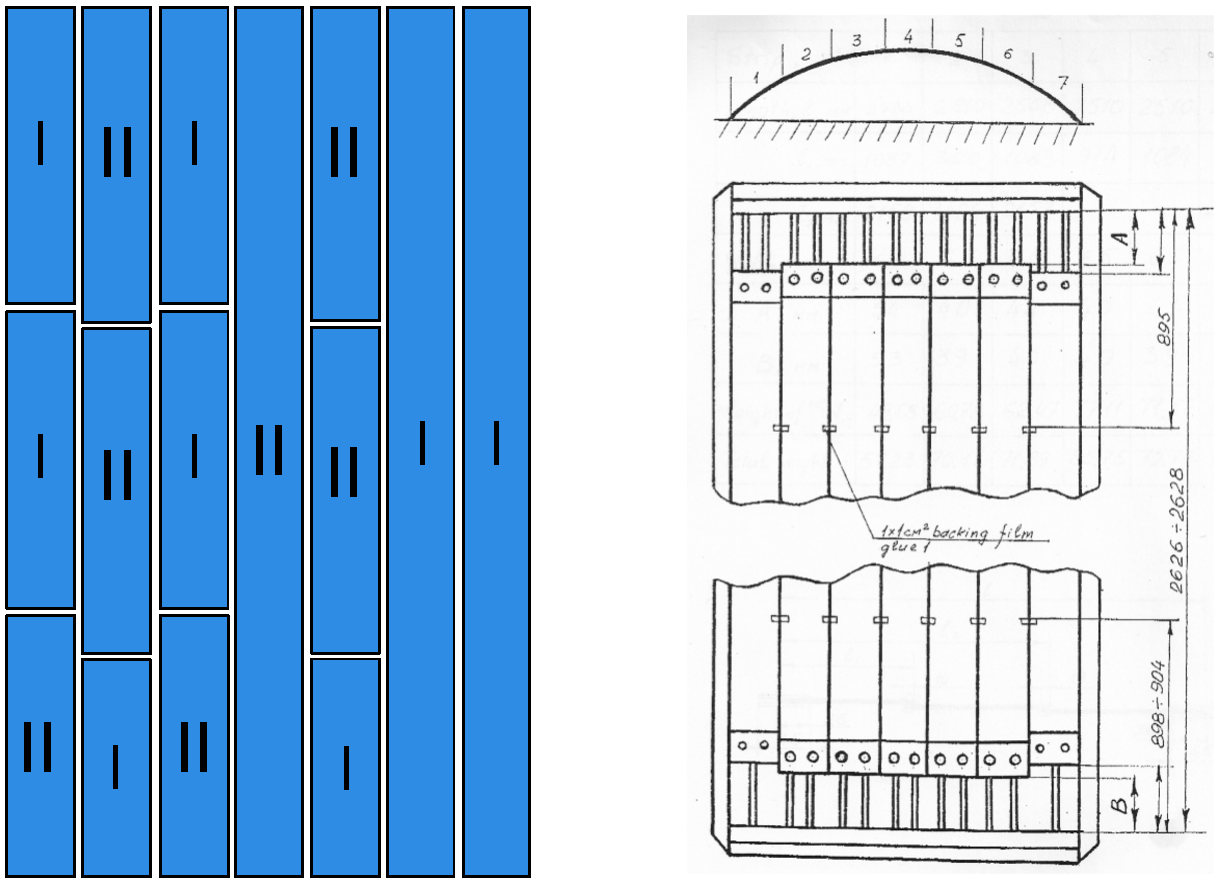
\includegraphics[height=7.7cm]{pictures/Chap6/schemaFoil_v2.pdf}
\centering
\caption{Left : Schematic view of the sector 18. The seven cadmium foils are divided in smaller pieces and glued together. The labels I and II correspond to the different \Cd~productions. Right : Drawing of the strips of cadmium showing the plexiglass clips that attach the foil to the support structure. The small pieces of backing film used to join the individual strips to one another.}
\label{CdFoil}
\end{figure}


\NI Before to be introduced in the detector, the radioactive contaminations of the cadmium foils have been measured thanks to High Purity Germanium detector (HPGe). The results of the different contaminations are summarized in Table \ref{TableContaminationMeasurements}.


\bigskip


\begin{table}[h!]
\begin{center}
\begin{tabular}{c|c|c|c|c|c|c|c|c}
   \toprule
   Source  & Mass [g] & Exposure [h] &\multicolumn{6}{c|}{Activity [mBq/kg]} \\
   \midrule[0.05cm]
           &          &              & $^{\text{40}}$K &  $^{\text{235}}$U &  $^{\text{234}}$Th & $^{\text{214}}$Bi  & $^{\text{228}}$Ac & $^{\text{232}}$Tl \\[0.1cm]
   Type I  & 257      & 778          & < 13     & < 0.5      & < 12        & < 1.5                  & < 2        & < 0.5 \\
   Type II & 299      & 368          & < 20     & < 1        & < 56        & < 1.7                  & < 4        & < 0.83 \\
   \bottomrule
\end{tabular}
\caption{Measurements of the cadmium source foils (including mylar support) realized with HPGe detector.}
\label{TableContaminationMeasurements}
\end{center}
\end{table}


\FloatBarrier


\subsection{Tracker}


\NI The NEMO-3 tracker provide three-dimensional tracking of charged particles to measure the decay properties of $\beta\beta$ events. It is composed of 6180 vertical drift cells operating in Geiger mode, which surround the source foils on both sides. The cells are arranged into nine different layers and divided into a 4-2-3 configuration, as shown in Figure~\ref{TrackerNEMOView}. The four layers close to the source allow a good reconstruction of the $\beta\beta$ vertex location to the source foil, the two middle layers provide the measurement of the track curvature and the three final layers are used to determine the interaction point of the calorimeter block. The gaps between the layers correspond to the location of calorimeter modules on top and bottom, which increase the coverage of the detector.


\bigskip


\begin{figure}[h!]
\begin{center}
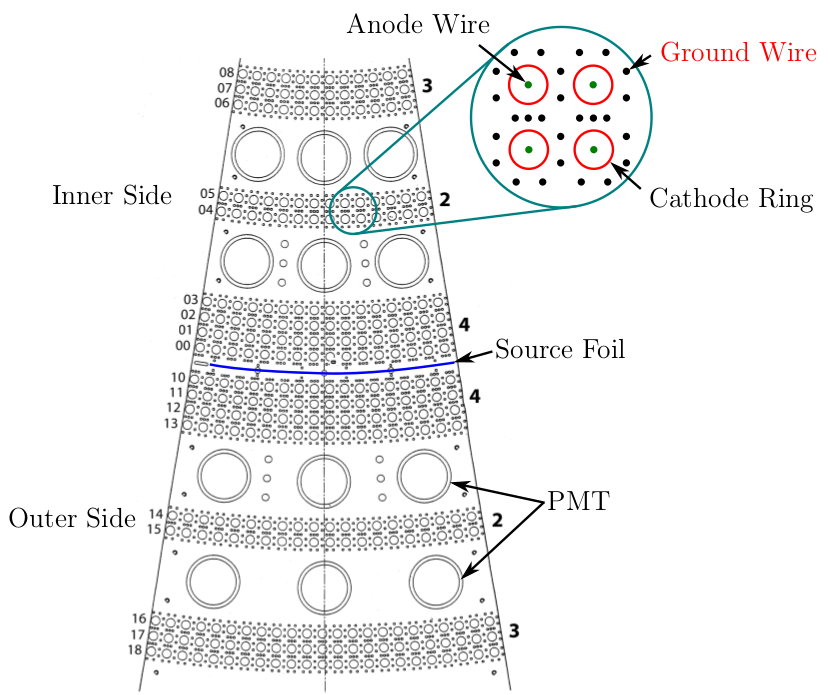
\includegraphics[scale=0.30]{pictures/Chap3/TrackerNEMOview.png}
\caption{Left : The 4-2-3 configuration of the Geiger cells in a NEMO-3 sector The 12 large rings represent the location of the light guides installed in the support structure to couple the scintillators to the PMTs. Right : Geiger
wiring of four elementary Geiger cells.}
\label{TrackerNEMOView}
\end{center}
\end{figure}


\NI An elementary cell (Figure~\ref{GeigerCellNEMO3}) is 2.7~m long and 3~cm in diameter, consisting of a central anode wire surrounded by eight ground wires. Four of these cathode wires are shared between the neighbouring cells, as shown in Figure~\ref{TrackerNEMOView}. This has the advantages from a radiopurity point of view and also minimizes the scattering inside the tracker. An extra ground wire have been added between the layers to avoid electrostatic cross talk. The wires are made of stainless steel, 2.7~m long and 50~$\mu$m in diameter. Copper cathod rings located at the top and bottom of the anode wires collect signals. These rings are 3~cm long a 2.3~cm in diameter.


\bigskip


\NI The gas inside the tracker volume is a mixture of 95~\% of helium, 4~\% of ethanol, 1~\% of argon and 0.1~\% of water held at 10~mbar above atmospheric pressure. Helium is used as basis of the tracking gas, since it is a noble gas with a low atomic number, and which minimises multiple scatterings. When traversing the tracker, an electron from $\beta\beta$ decay only lost approximately 30~keV. To quench the photoionisation process, by absorbing UV photons, small quantity of ethanol is mixted with helium. The performance of the tracker is then improved by reducing the re-firing effect of one cell to another. Some argon is also introduced to the mixture to stabilize the plasma propagation. Finally, in the final year of the detector, very small amount of water vapour have been added in order to rejuvenate the ageing cells.



\begin{figure}[h!]
\begin{center}
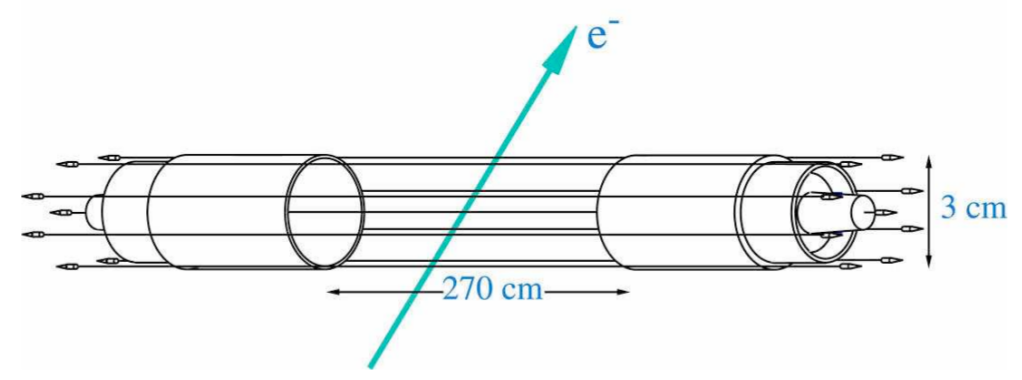
\includegraphics[scale=0.3]{pictures/Chap3/GeigerCellNEMO3.png}
\caption{Representation of an elementary Geiger cell in NEMO-3. The central anode wire of 270~cm length is surrounded by 8 ground wires. The cathod rings are shown at each end of the cell, 3~cm of diameter.}
\label{GeigerCellNEMO3}
\end{center}
\end{figure}


\NI When a charged particle crosses the tracking volume, the gas is ionised, producing He$^{+}$ ions and electrons. By applying a potential difference of about 1600~V between anode and cathode wires, these electrons drift towards the central anode and are accelerated, ionising more atoms. This create an avalanche that arrives at the anode wire and produces a signal. In this operating mode, a crossing charged particle creates $\sim$~6~electrons/cm. The drift speed is $\sim$~2.3 cm/$\mu$s, close to the anode, and $\sim$~1~cm/$\mu$s near the ground wires. The radial position of a particle can be reconstructed using the drift time drift and the globlal trigger (see Section ). During the electron avalanche, UV photons are induced which create a plasma. This plasma propagates along the length of the wire in both side at the speed of 6 to 7 cm/$\mu$s. The detection of this plasma by the cathode rings give information on the longitudinal position of a crossing particle. For 1~MeV electron, the average hit resolution of a cell is 0.5~mm  on  the  transversal plane and 8.0~mm on the longitudinal axis.


\subsection{Calorimeter}


\NI The roles of the NEMO-3 calorimeter are to measure the energy of the incindent particles, provide timing informations of particles in an event, and give a fast trigger signal. The calorimeter surrounds the tracking chambers on all sides. It consists of 1940 separated optical modules. Each optical module is made of a scintillator block, two light guides and either a 3'' or 5'' PMT according its position in the detector. A schematic view of a NEMO-3 optical module is presented in Figure~\ref{CaloModuleNEMO3}.	


\begin{figure}[h!]
\begin{center}
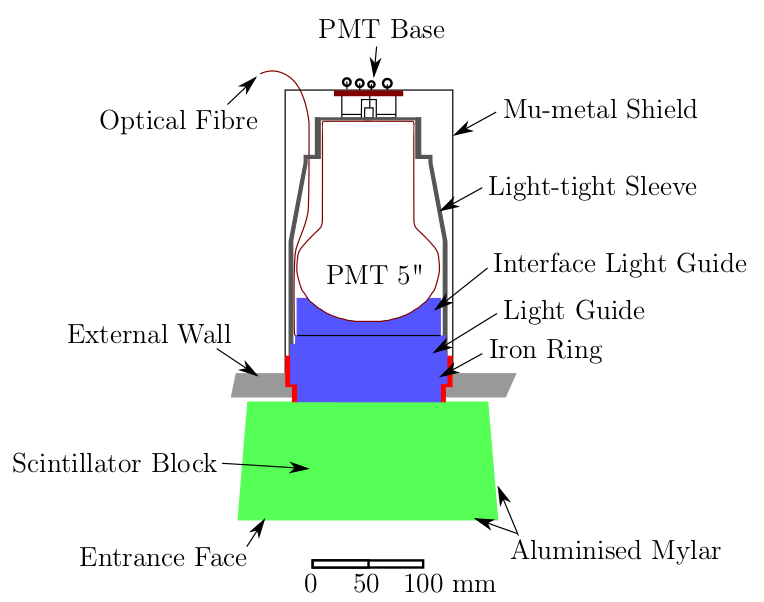
\includegraphics[scale=0.34]{pictures/Chap3/CaloModuleNEMO3.png}
\caption{One sector of NEMO 3 with details on the source foil, scintillator blocks and photomultipliers location.}
\label{CaloModuleNEMO3}
\end{center}
\end{figure}


\NI The scintillator blocks are mainly made of a styrene polymere, PST (C$_\text{6}$H$_\text{5}$CH=CH$_\text{2}$), doped with a scintillating agent, p-Terphenyl (PTP), and a wavelength shifter, 1.4-di-(5-phenyl-2-oxazoly) benzene (POPOP).  


\begin{figure}[h!]
\begin{center}
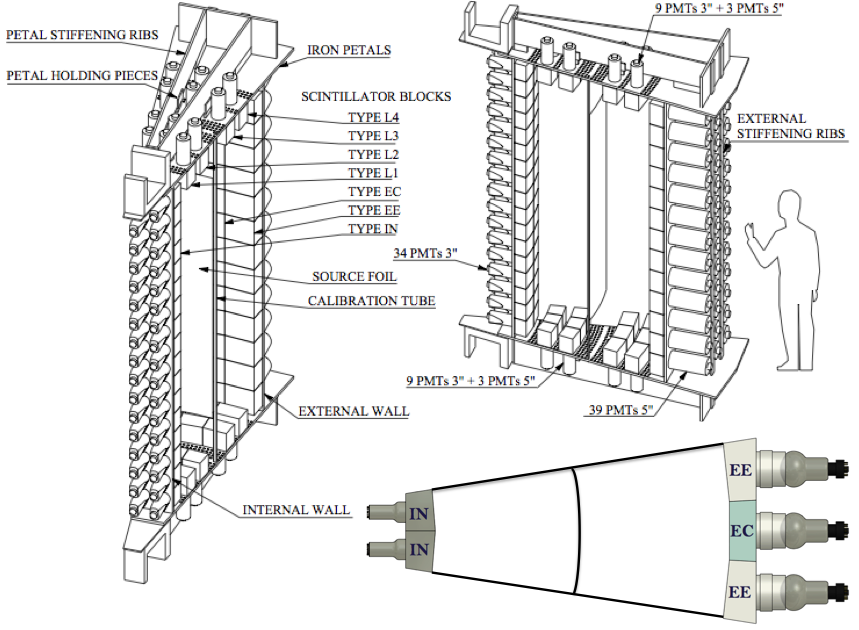
\includegraphics[scale=0.34]{pictures/Chap3/SectorDetailedPMTconfig.png}
\caption{One sector of NEMO 3 with details on the source foil, scintillator blocks and photomultipliers location.}
\label{SectorDetailedPMTconfig}
\end{center}
\end{figure}







\newpage

\newpage

\newpage

\newpage




\FloatBarrier





\subsection{Calorimeter}


\NI The NEMO-3 calorimeter is made of 1940 optical modules to measure the particle energy, make time of flight measurements and give a fast trigger signal. Each of optical module is made with a plastic scintillator, light guide and PMT (3'' or 5''). As shown in Figure~\ref{NEMO3Inside},  the scintillators blocks covered the inner and outer cylindrical walls of the detector, and also had limited coverage on the top and bottom (call petals). The gains of the PMTs have been adjusted to cover energies up to 12 MeV. The plastic scintillators have been chosen to minimize backscattering and for their radiopurity. The  calorimeter  provided  a  tim-ing  resolution  of $\sigma$ = 250~ps  while  the  energy  resolution  was $\sigma$E/E = 5.8~\%/$\sqrt{\text{E(MeV)}}$  for  the  scintillator coupled to 5'' PMTs, and 7.2~\%/$\sqrt{\text{E(MeV)}}$ for the scintillator equipped with 3" PMTs. 


\bigskip


\NI Two different kind of PMTs was used, the scintillator blocks of the internal walls and of the petals (except the petals close to the external wall) was coupled with R6091~3''~PMTs (1040 PMTs). These tubes are made of 12 dynodes and a flat photocathod. The blocks of the external wall and of the last petals were coupled to R6594~5''~PMTs (900 PMTs), having 10 dynodes and a hemispherical photocathode. A detailed schema of the location of the scintallator blocks in the NEMO-3 detector is presented in Figure~\ref{SectorDetailedPMTconfig}.


\smallskip




\NI The scintillator was directly in contact with the gas of tracker. In order to prevent a rapid aging of the PMT due to the helium-alcohol gas, the blocks were supported by a rigid frame which allows the PMTs to be outside. To fit the cylindrical geometry of NEMO-3, 7 different types of scintillator have been specialy designed. 


\bigskip


\NI The block are mainly made of a styrene polymere (C$_\text{6}$H$_\text{5}$CH=CH$_\text{2}$), with a mean Z of 3.7 per atom), 2~cm of this material is able to contain a up to 3~MeV electron. On the other hand, the mean Z is too low to optimise the photon interaction. The thickness of all the blocks have been set to 10~cm to obtain an efficiency for $\gamma$-ray detection of 50~\% at 500~keV. The chemical nature of the scintillator is a solid solution of a scintillating agent p-Terphenyl (PTP). Some 1.4-di-(5-phenyl-2-oxazoly) benzene (POPOP) is added in polystyrene to shift the wavelength for a better detection by the PMT ($\lambda \approx$ 420~nm). After many years of study, the final composition of the scintillation block have been chosen to be : 98.49~\% of polystyrene, 1.5~\% of PTP, and 0.01~\% of POPOP for the blocks of the walls and 98.75 \% of polystyrene, 1.2~\% of PTP, and 0.05~\% of POPOP for the petals blocks.


\bigskip


\NI The radiopurity of the scintillator blocks have measured to be 430 and 60 times better than the low radioactivity PMT (respectively in $^{\text{214}}$Bi and $^{\text{208}}$Tl). The blocks were finally wrapped with aluminized Mylar to not lose the scintillation light. A 60~mm thick light guide made of PMMA is used for the scintillator and PMT interface and to protect PMTs from helium. The light transmission through the guides is 98~\% in the wavelength range 380-420~nm.


\bigskip


\NI Based on analysis on NEMO-2 data, the dominant external background comes from the PMT. The development and the use of low radioactivity background is then crucial. For NEMO-3, the requirements for the PMT glass radioactivity was lower than 1.7~Bq/kg in $^{\text{40}}$K, lower than 0.83~Bq/kg in $^{\text{214}}$Bi and lower than 0.17~Bq/kg in $^{\text{208}}$Tl. The Hamamatsu company was chosen to produce the PMTs, with the radiopurity of their glass being 100 to 1000 times better than standard glass. Furthermore, the performances of their PMTs have been tested and meet the specifications : an energy resolution of 4~\% at 1~MeV, a time resolution of 250~ns at 1~MeV, a good linearity up to 4~MeV and a low dark current.  


\begin{figure}[h!]
\begin{center}
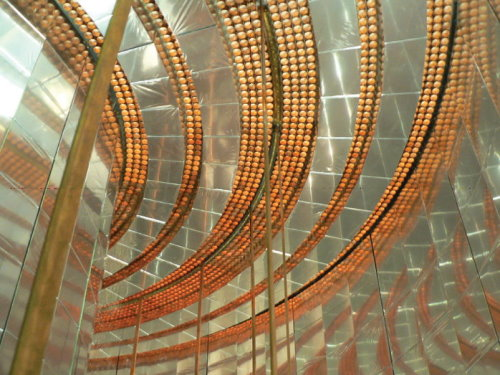
\includegraphics[scale=0.75]{pictures/Chap3/NEMO3Inside.jpg}
\caption{Inside view og the NEMO-3 wire chamber during disassembly. The reflective surfaces are the calorimeter walls and the copper parts support the Geiger cell wires.}
\label{NEMO3Inside}
\end{center}
\end{figure}



\NI Since the wires providing the high voltage of the PMTs are located inside the detector, they have to be made in radiopure materials. The PMT bases have been arranged with a progressive voltage divider in order to improve the linearity under high voltage conditions. All the PMT bases are supplied with 350~$\mu$A, the mean value of the high voltage is 1350~V for the 5'' PMT and 1800~V for the 3'' PMT. The length of the high voltage cables is the same 11~m with a positive tension (ground to the photocathode). In order to correct the different transit time (3 ns) between the two kind of PMT, the cable length are different for the output signals (11.3~m long for the 5'' PMT and 10.6~m long for the 3'' PMT). The 3 roles of the calorimeter are to measure the energy from the signal charge (ADC), measure the arrival time of the particles (TDC) and provide a quick trigger.


\FloatBarrier


\subsection{Magnetic coil and shielding}


\NI Despite NEMO-3 was located at LSM under 4800~m water-equivalent, which highly reduces the cosmic muon flux, the detector must be protected by different shieldings. Neutrons produced from ($\alpha$, n) reactions, cosmic muon spallation or spontaneous fission of uranium undergo neutron capture and produce high energy $\gamma$-rays. As seen in Section~ , these $\gamma$-rays are able to reproduce the $\beta\beta$ decay signal. Layers of passive shielding were installed around the detector to protect against the external neutron and $\gamma$-ray flux. A magnetic field allows positron/electron discrimation helps the identification of remaining external decay products.


\subsubsection{The magnetic coil}


\NI A solenoid magnet surrounding entirely the calorimeter produces a magnetic field of 25~Gauss parallel to the axis of the cylinder. The field is generated by running a current of $\sim$~ 30~A through a 5~tons copper coil of 5320 mm in diameter, 2713 mm high. Fans were used to cool the coil and the PMTs. A $\mu$-metal shielding is used to protect the PMTs from the magnetic field. 


\bigskip


\NI The magnetic field allows discrimination between $\beta\beta$ decay events and electron-positron (e$^+$e$^-$) pair from interactions of high energy $\gamma$-rays in the source foil. The rejection of the e$^+$e$^-$ pair is $\sim$~95~\% efficient at 1~MeV. 

\bigskip


\subsubsection{The shieldings}


\NI To suppress the neutron flux inside NEMO-3, a neutron shielding surrounds the detector. This shield consists of 20~cm of paraffin located below the central tower (not shown in Figure~\ref{NEMO3Detector}), 35~cm of borated water placed in tanks and 28~cm of wood above and below the detector end caps. Neutrons are thermalized by the paraffin, wood or water, and captured on boron. 


\bigskip

\NI To stop the $\gamma$-ray emitted in the neutron capture, a second shield made of iron is placed between the detector and the first shielding. This shield is made of 177 tonnes of iron, selected for its radiopurity, and is 20~cm thick.


\subsubsection{The anti-radon facility}


\NI Despite precautions taken to isolate the detector from the laboratory air with radon-tight seals, an excess of radon has been discovered after one year of data-taking. This high level of radon was due to leaks through the joints of the external shielding and calorimeter walls.


\bigskip


\NI To fix this problem, a anti-radon facility have been installed at the end of 2004. The facility is made of an hermetic polyethylene tent surrounding the entire detector, filled by radon-free air. The air of the laboratory was purified thanks to a radon trapping system using porous charcoal. When the air passes through the chacoal, the radon is trapped for a period of time allowing its decay. The output air is three order in magnitude poorer in radon than the incoming air.


\bigskip


\NI After the installation of the anti-radon facility, the level of radon inside NEMO-3 decreased by a factor $\sim$~6, see Figure~\ref{RadonByTime}. This reduction is much lower than the expected reduction, which is not completely explained. The two main hypotheses are that there is a higher radon level inside the tent that at the facility output, or a significant level of radon may be emanating from detector components. The two periods before and after the installation of the anti-radon facility are referred to as Phase~1 (February~2003 to September~2004) and Phase 2 (October 2004 to January 2011) respectively.

 
\begin{figure}[h!]
\begin{center}
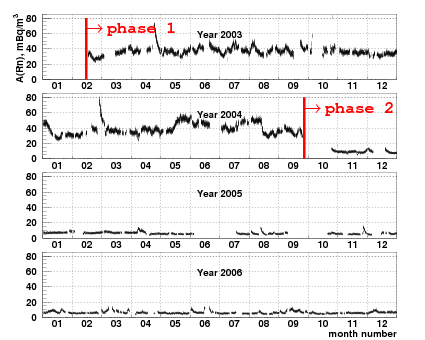
\includegraphics[scale=0.6]{pictures/Chap3/rn_bytime.png}
\caption{Radon activity measured in the NEMO-3 detector. The level of radon is reduced by a factor $\sim$~6. The time periods preceding and following the anti-radon facility are respectively referenced as Phase 1 and Phase 2.}
\label{RadonByTime}
\end{center}
\end{figure}


\FloatBarrier


\subsection{Electronics and DAQ}


\subsection{Calibration system}

\NI To distinguish true 0$\nu\beta\beta$ events from various background processes (2$\nu\beta\beta$ decay is only experimentaly differentiable from 0$\nu\beta\beta$ by energy), a good calorimeter energy resolution is important. Thus a robust calibration procedure is needed to ensure and monitor the response of the calorimeter and detect any changes over the lifetime of the experiment. The NEMO-3 solution is the use of radioactive sources introduced inside the detector during runs dedicated to calibration. The absolute energy scale is determined during these runs (approximately one day every month), but the rest of the time, a laser survey system control the stability of the optical modules. 


\bigskip


\NI To introduce different calibration sources into the detector each sectors was equiped with a vertical tube made of flattened copper located along the edge of the source foils. The sources were placed along a narrow delrin rod (3 per rod at z~=~-90, 0 and +90~cm), and introduced by the top of the detector (after the removal of some shields). The position of the sources have been chosen to obain an uniform illumination of the scintillator blocks. This system allow to place the calibration sources close the $\beta\beta$ foils, thus the electron trajectories are very similar to the expected tracks in $\beta\beta$ events.


\bigskip


\NI Some studies shown that the response of the calorimeter was not the same for electrons and photons due to a difference in light collection. The electrons directly interact at the entrance of the scintillator while the photons interact deeper in the block. As we are interested by the electrons, the choice was made to use $^{\text{207}}$Bi and $^{\text{90}}$Sr sources. Decay of $^{\text{207}}$Bi provides conversion electrons of 482 and 976 keV. In order to not saturate the detector, the activity of the 60 sources of $^{\text{207}}$Bi should not be too high, each source have an activity around 6~nCi (222~Bq). To have access energies up to 3~MeV or more, an additional calibration point is got using electrons from $^{\text{90}}$Y (daughter of $^{\text{90}}$Sr) and the end-point of the $\beta$ spectrum at 2.283~MeV.


\bigskip


\NI For timing calibration of the detector, sources of $^{\text{60}}$Co are employed. These sources emits two $\gamma$-ray in  coincidence with energies of 1332 and 1173 keV. With the dispersion of arrival times differences, the delays between the 1940 channels is established. The activity of these sources can be high since the tracker is not required for this calibration.


\bigskip


\NI To monitor the stability of the calorimeter between absolute calibration runs, a calibration system of laser have been developed. Its main objective is to daily check the absolute energy and time calibrations. The PMTs linearity between 0 and 12~MeV is also determined also as the time-energy relation. In order to accomplish all these measurements, the shape of the laser signal must be very similar to the one produced by an electron and the emitted light has to be known with a high accuracy (< 1~\%) and stay stable. 


\bigskip


\NI The lasers used was di-azote lasers (N$_\text{2}$) with a wavelength of 337~$\pm$~15~nm. The light beam was divided into two parts. The first is directly sent to a photocathode to monitor the laser light intensity. To mimic the electron signal, the second beam is shifted to 420~nm with two optical filters. The light is then sent to the calorimeter blocks via optical fibers. Six independant reference blocks were equipped with $^{\text{207}}$Bi sources allowing to monitor the laser intensity by measuring energies of both the laser and the 976 keV conversion electrons.


\bigskip


\NI The relation between the charge signal and the energy deposited in the block is linear up to 4~MeV, which matches to the $\beta\beta$ region (the higher Q$_{\beta\beta}$ is 4.27~MeV for $^{\text{48}}$Ca) : 


\begin{equation}
\text{E} = \text{a} \times \text{(C - P) + b} 
\end{equation}


\NI where E is the energy, C the ADC value of the scintillator and P the pedestral. The energy calibration contants a and b are determined with at least two points from calibration sources measurements. In the simulation, the energy resolution is parametrized as :


\begin{equation}
\text{FWHM}^\text{2} \text{(E)} = \text{d} \times \text{E} + \text{e}
\end{equation} 

\NI where d $\times$ E coming from statistical fluctutations of the number of photoelectron arriving at the anode and of the number of scintillation photons. The parameter e represents the instrumental aspects independant of the energy.


\bigskip


\NI During the calibration phase using laser system, the last run is used to provide a reference energy for each optical module. In case the corrected gain (obtained with the laser system) is different from the gain get from $^{\text{207}}$Bi calibration sources a correction factor is applied.


\bigskip


\NI The cable length differences, the different geometry of the guide light and scintillator blocks or different PMT transit time can be responsible of different temporal response for two particle emitted in coincidence. In order to correctly calculate the time of flight of the particles and synchronize all the optical modules calibration sources of $^{\text{60}}$Co are used (2 $\gamma$-rays emitted in coincidence at 1332 et 1173 keV). Several runs of calibration changing the location of the sources have been taken.


\bigskip    


\NI Finally, thanks to the laser system, the time-energy dependance can be modeling by :


\begin{equation}
\text{t (C)} = \text{p}_\text{1} - \frac{\text{p}_\text{2}}{\text{p}_\text{3} \sqrt{\text{C}} + \text{p}_4}
\end{equation} 


\NI where C is the ADC value, all the other parameters ($p_i$) can be determined with the laser system in range [0-12]~MeV.


\FloatBarrier

\subsection{Results and measurements}


\NI After 5.25 years of data taking, NEMO-3 have been stopped and disassembled. The results on the searches for 2$\nu\beta\beta$ and 0$\nu\beta\beta$ are gathered in Table~\ref{tab:SummaryDecayRateNEMO3}. Most of these decay have been measured only by NEMO-3 or constitute the world best limits. The studies of the decays via the excited states and 0$\nu$4$\beta$ is also possible with the NEMO-3 detector.


\NI \textcolor{red}{ajouter les recherches concernant les états excités.}

\begin{table}[h!]
\centering
\begin{tabular}{c|c|c|c}
Isotopes & T$_{\text{1/2}}^{\text{2}\nu}$ [y] at 90 \% C.L. & T$_{\text{1/2}}^{\text{0}\nu}$ [y] at 90 \% C.L. & m$_{\beta\beta}$ [eV] \\
\toprule
$^{\text{100}}$Mo \cite{NEMO3:Mo100} & [7.1 $\pm$ 0.5] $\times$ 10$^{\text{18}}$ & > 1.1 $\times$ 10$^{\text{24}}$ & < [0.33 - 0.62]  \\[0.1cm]
$^{\text{82}}$Se \cite{NEMO3:Se82} & [10.07 $\pm$ 0.14 $\pm$ 0.54] $\times$ 10$^{\text{19}}$ & > 2.5 $\times$ 10$^{\text{23}}$  & < [1.2 - 3.0]  \\[0.1cm]
$^{\text{130}}$Te \cite{NEMO3:Te130}& [7.0 $\pm$ 0.9 $\pm$ 1.1] $\times$ 10$^{\text{20}}$ & > 1.3 $\times$ 10$^{\text{23}}$  & - \\[0.1cm]
$^{\text{116}}$Cd \cite{Arnold2016bed}& [2.74 $\pm$ 0.04 $\pm$ 0.18] $\times$ 10$^{\text{19}}$ & > 1.0 $\times$ 10$^{\text{23}}$  & < [1.4 - 2.5]  \\[0.1cm]
$^{\text{150}}$Nd \cite{NEMO3:Nd150}& [9.34 $\pm$ 0.22 $\pm$ $^{+\text{0.62}}_{-\text{0.60}}$] $\times$ 10$^{\text{18}}$ & > 2.0 $\times$ 10$^{\text{22}}$  & [1.6 - 5.3] \\[0.1cm]
$^{\text{96}}$Zr  \cite{NEMO3:Zr96}& [2.35 $\pm$ 0.14 $\pm$ 0.16] $\times$ 10$^{\text{19}}$ & 9.2 $\times$ 10$^{\text{21}}$  & - \\[0.1cm]
$^{\text{48}}$Ca \cite{NEMO3:Ca48} & [6.4 $\times$ $^{+\text{0.7}}_{-\text{0.6}}$ $^{+\text{1.2}}_{-\text{0.9}}$] $\times$ 10$^{\text{19}}$ & 2.0 $\times$ 10$^{\text{22}}$  & < [6.0 - 26] \\[0.1cm]
\bottomrule
\end{tabular}
\caption{Summary of the different half-lives measured for isotopes introduced in NEMO-3.}
\label{tab:SummaryDecayRateNEMO3}
\end{table}


\FloatBarrier


\section{SuperNEMO}\label{sec:SuperNEMO}


\NI Based on the NEMO-3 experiment, SuperNEMO is a new detector among the next generation searching for 0$\nu\beta\beta$. The strategy consists to take advantage of the previous detectors and increase the isotope mass of an improve the radiopurity. A total of 100~kg of isotopes could be studied allowing to reach 10$^{\text{26}}$~years on the 0$\nu\beta\beta$ process. The SuperNEMO project is composed of 20 identical modules. Thanks of several years of R\&D, great improvement have also been made concerning the energy resolution of the calorimeter. Table~\ref{tab:DifferenceNEMO3-SuperNEMO} summarizes the difference in performance for NEMO-3 detector and SuperNEMO project.


\begin{table}[h!]
\centering
\begin{tabular}{c|c|c}
      & NEMO-3 & SuperNEMO \\
\toprule
Mass~[kg] (main isotopes)           & 7 ($^{\text{100}}$Mo)         & 100 ($^{\text{82}}$Se)        \\[0.1cm]
 T$_{\text{1/2}}^{\text{2}\nu}$ [y] & 7.2 $\times$ 10$^{\text{18}}$ & 9.9 $\times$ 10$^{\text{19}}$ \\[0.1cm]
\midrule
Energy resolution & & \\
FWHM at 1~MeV                       & 15~\%                         & 8~\%                          \\[0.1cm]
FWHM at 3~MeV                       & 8~\%                          & 4~\%                          \\[0.1cm]
\midrule
Source radiopurity & & \\
A($^{\text{208}}$Tl)               & $\sim$ 100 $\mu$Bq/kg         & $<$ 2 $\mu$Bq/kg               \\[0.1cm]
A($^{\text{214}}$Bi)               & < 300 $\mu$Bq/kg              & < 10 $\mu$Bq/kg                \\[0.1cm]
\midrule
Level of radon A($^{\text{222}}$Rn)& $\sim$ 5.0 mBq/m$^\text{3}$ y   & < 0.1 mBq/m$^\text{3}$ y     \\[0.1cm]
\midrule
Sensitivity after 5~y of data taking & T$_{\text{1/2}}^{\text{0}\nu}$ > 10$^{\text{24}}$ & T$_{\text{1/2}}^{\text{0}\nu}$ > 10$^{\text{26}}$     \\[0.1cm]
\bottomrule
\end{tabular}
\caption{Summary of the difference in performance for NEMO-3 detector and SuperNEMO project.}
\label{tab:DifferenceNEMO3-SuperNEMO}
\end{table}  

\FloatBarrier


\subsection{The SuperNEMO demonstrator module}


\NI Before to build the 20 modules and in order to verify and validate the low level of background at large scale, the collaboration is building a first module called demonstrator module. This module will also serve to validate the technological choices (detection efficiency of the tracker, energy resolution of the calorimeter and source foil purification process). This module will contain 7~kg of $^{\text{82}}$Se in the form of thin source foils for physics study ($\sim$ 6.0 $\times$ 10$^{\text{24}}$~years on the 0$\nu\beta\beta$ process). 


\begin{figure}[h!]
\begin{center}
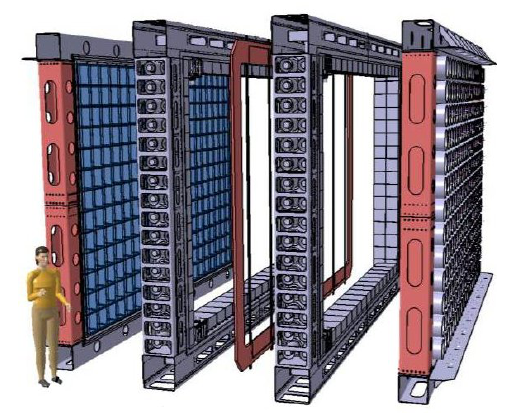
\includegraphics[scale=0.55]{pictures/Chap3/snemomodule.png}
\caption{Exploded view of one module of SuperNEMO. Thin source foils of $^{\text{82}}$Se are place at the center of the detector. 2 trackers modules made of 2034 Geiger cells reconstruct the electron tracks. 2 calorimeters walls measure the electron energies.}
\label{SuperNEMOexplodedView}
\end{center}
\end{figure}


\NI Figure~\ref{SuperNEMOexplodedView} presents a exploded view the demonstrator module. A planar geometry have been chosen. A central frame supports the thin foils of $\beta\beta$ emitters. The foils are sandwiched surrounded by the 2 tracker modules and 2 calorimeter walls inside water and iron shieldings. 


\FloatBarrier


\subsection{$^{\text{82}}$Se source foils}


\NI To choose the isotope of the demonstrator module a compromise must be find between many parameters. The choice have been made to use $^{\text{82}}$Se because of  its long 2$\nu\beta\beta$ half-life (to limit the irreducible background from 2$\nu\beta\beta$ in the search for 0$\nu\beta\beta$), its great Q$_{\beta\beta}$ (to limit the background coming from natural radioactivity) and a possible enrichment on a large scale. Some studies have been made for a possible used of $^{\text{150}}$Nd and $^{\text{48}}$Ca in a second phase of SuperNEMO.


\bigskip


\NI The source is divided in 36 foils (34 with 13.55 cm width and 2 with 12.5 cm width). A drawing of the source foil geometry can be found in Figure~\ref{SuperNEMOFoils}. The width of the total source is 485.7 cm, its height is 270.0 cm for a total surface of 131 139 cm$^\text{2}$ and a mean density of 55 mg/cm$^\text{2}$.


\begin{figure}[h!]
\begin{center}
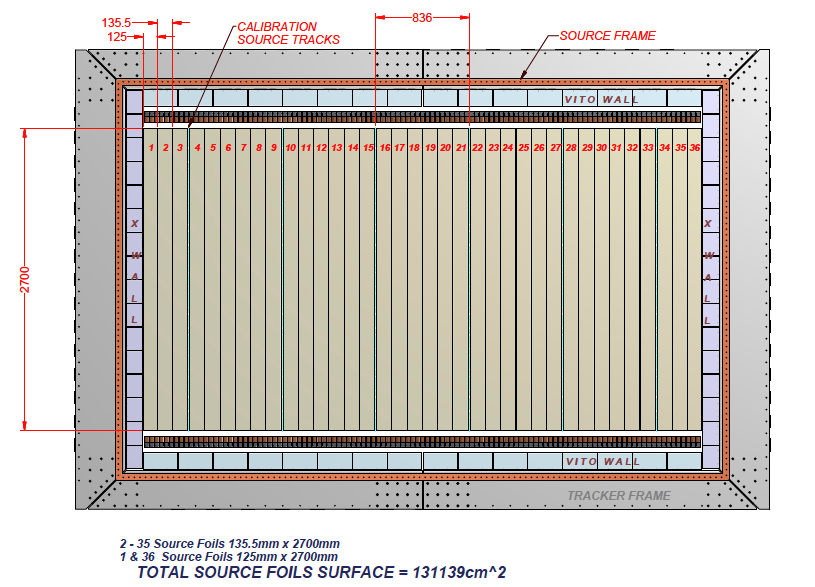
\includegraphics[scale=0.33]{pictures/Chap3/foil.png}
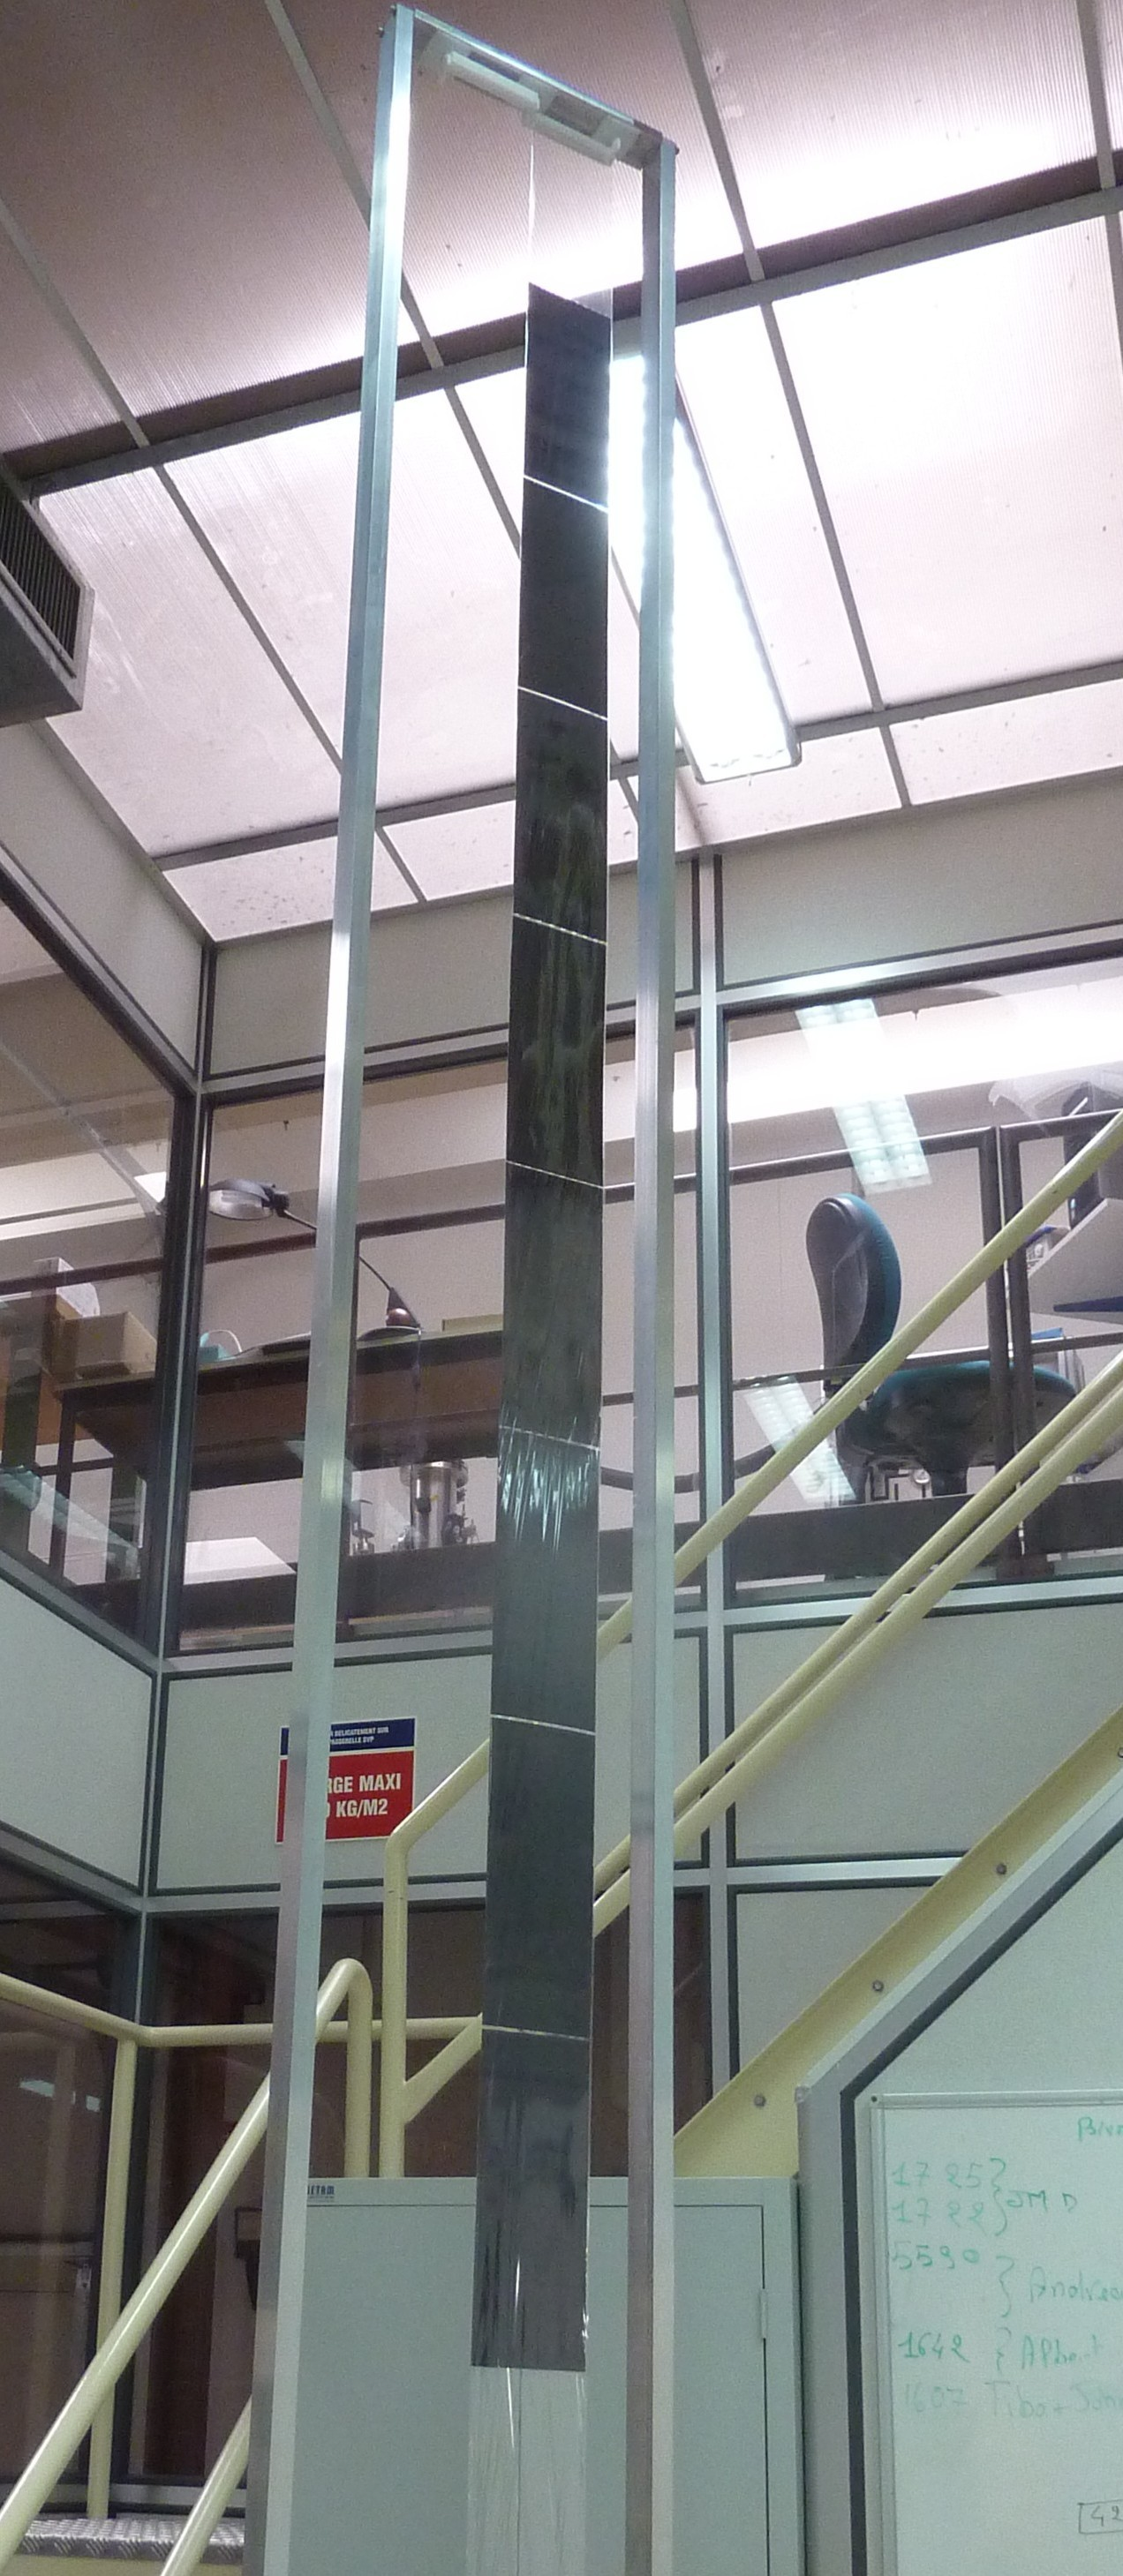
\includegraphics[scale=0.075]{pictures/Chap3/P1090162.JPG}
\caption{Left : Selenium source foils final geometry, it is divided in 36 foils
(34 with 13.55 cm width and 2 with 12.5 cm width). Right : Picture of one strip : the Se+PVA pad is surrounded by two raw mylar foils. These
two raw mylar foils are welded.} 
\label{SuperNEMOFoils}
\end{center}
\end{figure}


\NI The selenium is under a powder form. This powder is mixed with a radiopure glue (PolyVinyl Alcohol : PVA) and ultrapure water to obtain a liquid paste. This paste is spread out between two a mylar sheet of 10~$\mu$m thick pierced by micro-holes. These micro-holes allow a good coupling between the paste and the foil and facilitate evaporation. Unfortunately, these holes was made at JINR Dubna using a ions beam which can contaminate the source foil. It is in this optic that a new foil fabrication procedure have been proposed and studied in R\&D. The second method consists of unfolding the selenium foil and cut it into pads. These pads are then inserted into two mylar foils joined with a weld (mylar without micro-holes so not irradiated). More detailled on source foil optimisation will be given in Chapter~4.


\bigskip


\NI To reach a sensitivity of 10$^{\text{26}}$~years, the required level of radiopurity is 2$\mu$Bs/kg and 10$\mu$Bs/kg for $^{\text{208}}$Tl and $^{\text{214}}$Bi. The selenium must be enriched and purified. Two purification methods have been studied  : a chemical one and by distillation. 

\ifx
aa
\fi

\FloatBarrier


\subsection{The BiPo detector}


\NI The measurement of very low levels of radiopurity is not possible using germanium detector, as is generally the case. Their sensitivity is around 50 $\mu$Bq/kg for the level of $^{\text{208}}$Tl. The NEMO collaboration decided to develop and build a detector dedicated to the measurement of very low contaminations (in $^{\text{214}}$Bi and $^{\text{208}}$Tl ) of the source foils.


\bigskip  


\NI To identify $^{\text{214}}$Bi and $^{\text{208}}$Tl, the BiPo detector~\cite{BiPoDetector} is based on the observation of the so-called BiPo events. In the decay chain of $^{\text{238}}$U and $^{\text{232}}$Th, BiPo events are cascades of $\beta$ and delayed $\alpha$ decays. For example, as shown in Figure~\ref{BiPoDecayChain}, in uranium decay chain, $^{\text{214}}$Bi is a $\beta$ emitter decaying to $^{\text{214}}$Po, which is itself an $\alpha$ emitter with a characteristic half-life of 164~$\mu$s.


\begin{figure}[h!]
\begin{center}
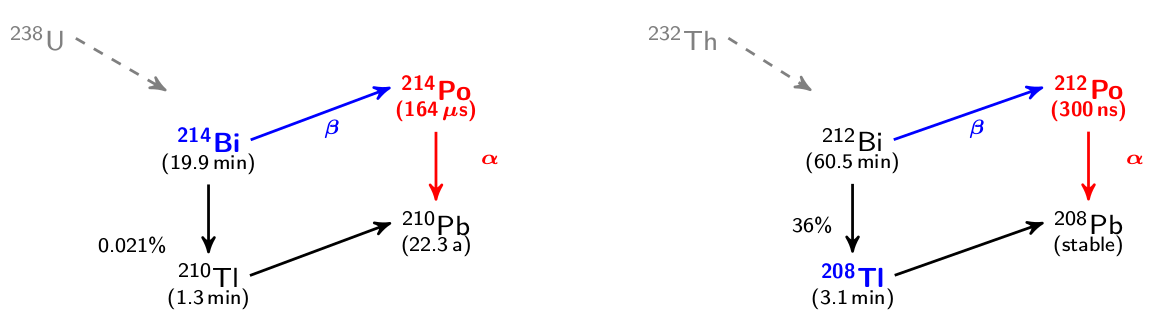
\includegraphics[scale=0.33]{pictures/Chap3/BiPoDecayChain.png}
\caption{The $^{\text{214}}$Bi$^{\text{214}}$Po and $^{\text{212}}$Bi$^{\text{212}}$Bi cascades used to measure the $^{\text{214}}$Bi and $^{\text{208}}$Tl contaminations.}
\label{BiPoDecayChain}
\end{center}
\end{figure}


\NI In order to detect the e$^-$ and $\alpha$ particles, the sources are installed between two thin ultra-radiopure plastic scintillators couplingto low radiative PMTs, as schematized in Figure~\ref{BiPoEvent}. 

\begin{figure}[h!]
\begin{center}
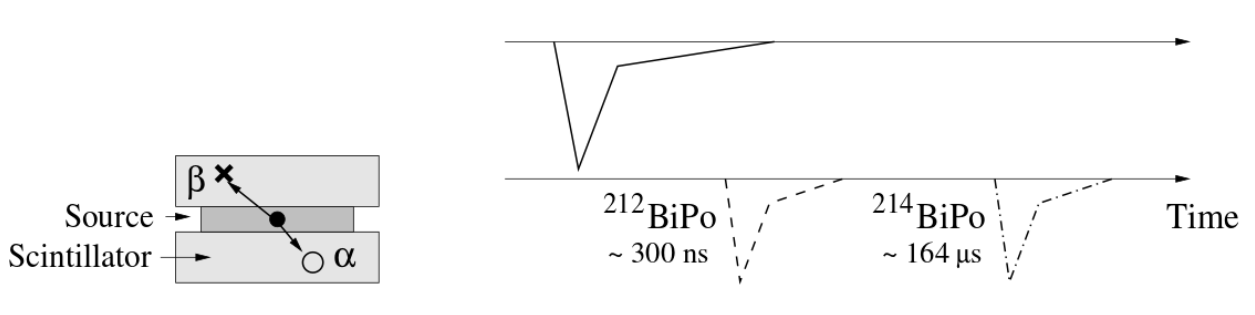
\includegraphics[scale=0.3]{pictures/Chap3/BiPoEvent_2.png}
\caption{Left : schematic view of the BiPo detection technique with the source  foil  inserted  between  two  plastic  scintillators  plate. Right : scintillation signal waveforms acquired for a BiPo event. The prompt signal  and  the  delayed signal observed  by  the  top  and  bottom scintillators respectively are schematically shown.}
\label{BiPoEvent}
\end{center}
\end{figure}


\NI The BiPo detector have been installed in 2012 at Canfranc Underground Laboratory in Spain. It is made of 2 identical modules, each of them containing 40 scintillator blocks (coupled with 5'' PMTs). Each optical module covers an aera of 30 $\times$ 30 cm$^\text{2}$, as presented in Figure~\ref{BiPoDetector}. This segmentation allows detection of possible hot spots on the foil. 


\begin{figure}[h!]
\begin{center}
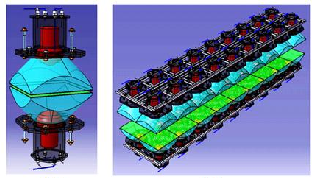
\includegraphics[scale=1.1]{pictures/Chap3/snemo_bipo.png}
\caption{Left : Pair of sub-modules coupled face to face. The green part represents the thin scintillators. The optical guides appear in blue and the PMTs in red. Right : assembly of the 40 optical sub-modules.}
\label{BiPoDetector}
\end{center}
\end{figure}


\bigskip


\NI In a first step, the detector took data without any foils to measure its own level of background. The results of 0.16~$\mu$Bq/m$^\text{2}$ in $^{\text{214}}$Bi and 1.28~$\mu$Bq/m$^\text{2}$ in $^{\text{208}}$Tl allow to reach the expected sensitivity (10 and 2~$\mu$Bq/kg in $^{\text{214}}$Bi and $^{\text{208}}$Tl) in few month of data taking.

\FloatBarrier


\subsection{Tracking volume}


\NI The tracking volume of SuperNEMO consists of 2 tracker modules made of 9 layers of 113 Geiger cells (for a total of 2034 Geiger cells). Each module is divided into 2 cassettes (for a total of 4 cassettes called C0, C1, C2 and C3) and mesure 5~m long, 3.4~m high and 40~cm depth. The tracker cells have been built and tested in Manchester before being transport at LSM.


\bigskip


\NI The commissioning of the first cassette used cosmic muon events with scintillator planes below the tracker volume 
acting as a trigger. A picture of a cassette and cosmic muon event is shown in Figure~\ref{SnemoTracker}. Of the 2034 tested cells, 23 are considered as bad (self trigger or plasma block). The proportion of operational channels is 98.9~\%. 


\bigskip


\NI During the R\&D phase a great care have been taken in order to drastically reduce the presence of radon inside the tracking volume. Based on the NEMO-3 analysis, 2 main reasons have been identified : the emanation of radon coming from the tracking device materials and a bad impermeability of the seals closing the volume (easy diffusion of the radon coming from PMTs).


\bigskip

\NI During the R\&D phase, different points have been studied to improve the wire chamber compared to NEMO-3 : 


\begin{itemize}
\item now, the wire chamber is isolated from the rest of the detector with a nylon radon-tight film.


\item Free-radon air will be introduced very close to the PMT to avoid high radon concentration. Futhermore, the entire detector will be inside a radon clean tent.


\item To maintain the tracking properties of the detector, the mixture ratio of the gas must be kept constant 
(95~\% Helium, 4~\% Ethanol and 1~\% Argon). A gas system ensures minxing and sends the gas into the detector. Great improvement have been done to purify the tracker gas. The helium can be easily purify using a coal traps.


\item all the materials placed inside the tracker volume are tested and measured in germanium detector. Emanation measurements are realized on each cassette to check that the mechanical processes have not introduced contaminations. The results of these measurements are summarized in Table~\ref{tab:RadonEmanation}. Extrapolated to full demonstrator, the value of 0.21~mBq/m$^{\text{3}}$ is obtain at nominal flowrate (0.12~mBq/m$^{\text{3}}$ when flushed at 1m$^{\text{3}}$/hr). 
\end{itemize}


\begin{figure}[h!]
\begin{center}
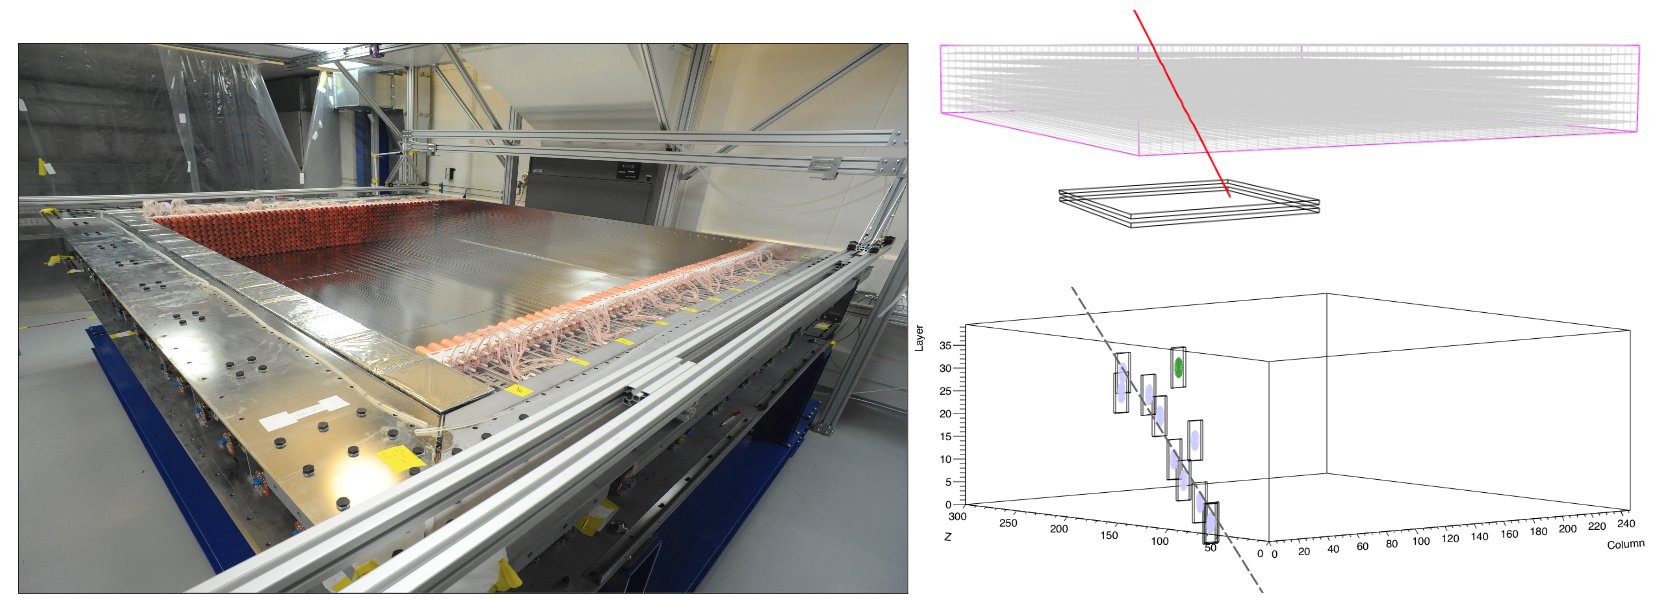
\includegraphics[scale=0.25]{pictures/Chap3/TrackerTestCosmic.png}
\caption{Left : picture of one of the four cassette fully assembled. The cassette is set horizontally, later in the SuperNEMO demonstrator, the Geiger cells will be vertical, parallel to the source foil. The copper part are the end-caps supporting the wires. Top right : simulation of a cosmic muon crossing throught the tracker. Bottom right : real event of a cosmic muon crossing the tracker.}
\label{SnemoTracker}
\end{center}
\end{figure}


\begin{table}[h!]
\centering
\begin{tabular}{c|c}
Cassette & Radon emanation \\
\toprule
C0 & 11.37 $\pm$ 1.44~mBq \\
C1 & 15.26 $^{+\text{2.5}}_{\text{4.0}}$~mBq \\
C2 & 3.28 $\pm$ 1.39~mBq \\
\bottomrule
\end{tabular}
\caption{Summary of the emanation measurements of the different cassette. The C4 have not been measured.}
\label{tab:RadonEmanation}
\end{table}


\NI The tracker volume will be coupled with a magnetic field (parallel to the source foil) for charge discrimination. Some studies have been realized to optimize its value (probably 25~G will be applied). 



\FloatBarrier

\subsection{Calorimeter}


\NI The calorimeter of the SuperNEMO demonstrator is composed of 712 optical modules distributed in 6 walls : 


\begin{itemize}

\item 2 main walls on opposite sides of the of the source foil faces. Each main wall contains 260~polystyrene cubic scintillator  blocks (256~mm $\times$ 256~mm $\times$ 194~mm) coupled to 8'' low radioactive PMT (R5912-03) which have a quantum efficiency between 35 and 45~\% at 420~nm. A main difference with the NEMO-3 blocks is that the PMT is directly coupled to the scintillator block, no light guide is used as it is shown in Figure~\ref{SnemoOpticalModule}. Thanks to this new design the energy resolution is highly improved (FWHM of 8~\% at 1~MeV).


\item 2 $\gamma$-veto to cap the top and the bottom of the detector containing 64~plastics scintillator blocks (210~mm $\times$ 200~mm $\times$ 145~mm) coupled to 5'' PMTs (R6594). 

\item 2 x-walls to cap the sides made of 32~plastics scintillator blocks (290~mm $\times$ 304~mm $\times$ 145~mm) also coupled to 5'' PMT.

\end{itemize}


\begin{figure}[h!]
\begin{center}
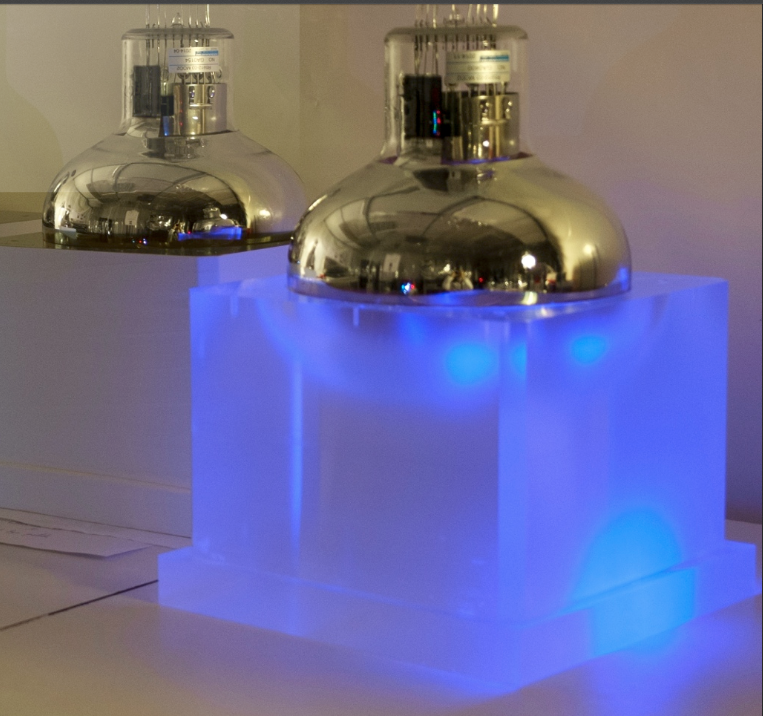
\includegraphics[scale=0.25]{pictures/Chap3/calo_1.png}
\caption{Optical module composing the calorimeter before to be wrapped into teflon and mylar. The scintillator block is directly coupled to the PMT.}
\label{SnemoOpticalModule}
\end{center}
\end{figure}


\NI To improve the light collection, all the blocks are wrapped into teflon for each block sides except the entry face which is covered by 6~$\mu$m of aluminized mylar.


\bigskip


\NI Figure~\ref{SnemoCaloFrontView} is a picture of the SuperNEMO main wall during its construction at LSM. For lack of 8'' PMTs, all the blocks in the top and bottom rows of the walls are coupled with 5'' PMTs.


\begin{figure}[h!]
\begin{center}
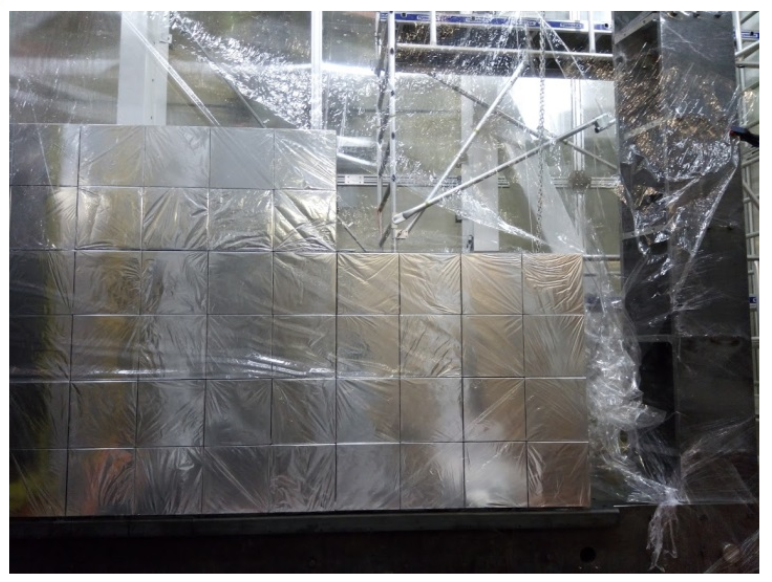
\includegraphics[scale=0.5]{pictures/Chap3/FrontViewCalo.png}
\caption{Front view of one main wall during its construction. The wall is built by assembling the bricks (8 by 8).}
\label{SnemoCaloFrontView}
\end{center}
\end{figure}

\FloatBarrier


\subsection{Calibration system}


\NI As it was the case in NEMO-3, 2 systems are used to calibrate the detector. Monthly, via a system of weights and stepper motors, $^{\text{207}}$Bi sources will be introduced inside the detector to calibrate the absolute energy scale. Between these dedicated runs, a light injection system has been developed to monitor the response and the linearity of the optical modules.


\bigskip


\NI The light injection system (LI) injects pulsed LED light into each scintillator blocks via optical fibers. A schematic view of the LI system is presented in Figure~\ref{LIschema}. Areference optical module is used to monitor the light level against a $^{\text{241}}$Am source. The 20 UV LEDs and the reference PMT are housed in a light-tight rack. The pulse height spectra recorded in a test optical module and reference block are presenter in Figure. 

\bigskip
\begin{figure}[h!]
\begin{center}
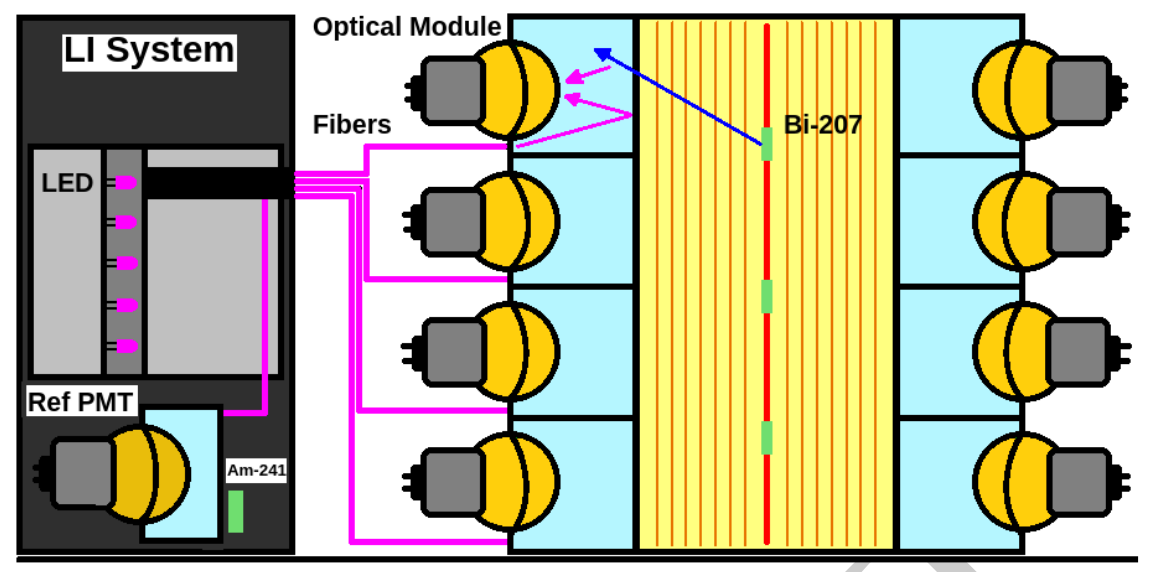
\includegraphics[scale=0.3]{pictures/Chap3/LIschema.png}
\caption{Schematic representation of the light injection system. Installed in an independant rack, a pulser will send into each optical module UV light via optical fibers. A reference PMT coupled to an americium source is used to control the light level.}
\label{LIschema}
\end{center}
\end{figure}


\NI To study how the LI system will be able to monitor and calibrate between $^{\text{207}}$Bi runs, the initial position of the 976~keV peak is used. The goal is to predict where it would be shifted to at a latter time using only the later LED peaks seen and the $^{\text{241}}$Am. Figure shows the ratio between the expected and the obserced signal, even with some jumps, the response of the optical module can be predicted within 1~\%.

\bigskip
\begin{figure}[h!]
\begin{center}
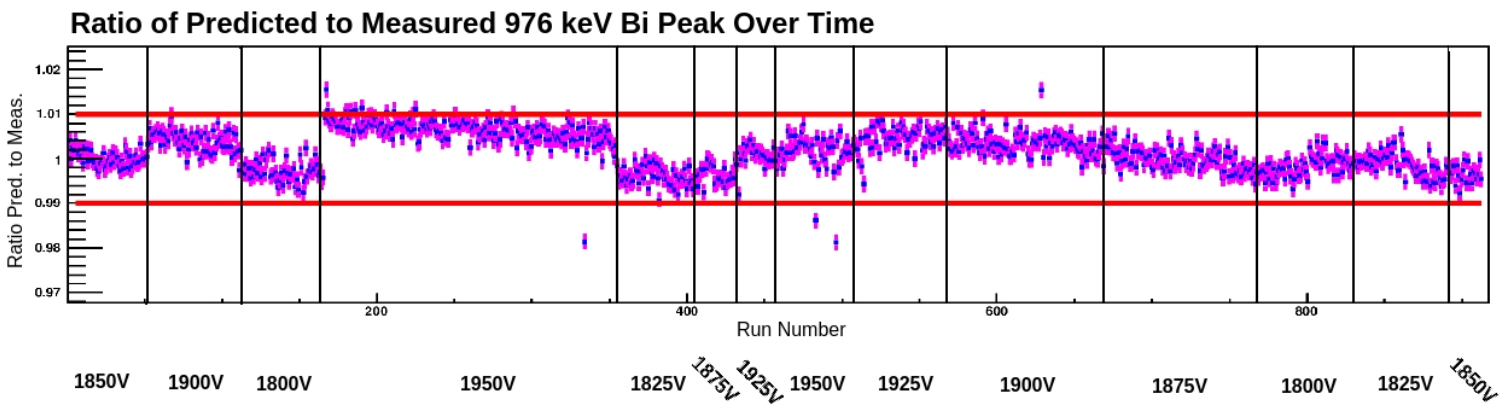
\includegraphics[scale=0.25]{pictures/Chap3/RatioPredictionLI.png}
\caption{Ratio of the predicted to measured peak position for the 976~keV $^{\text{207}}$Bi electron. The ratio deviates by not more than 1~\% as shown by the red lines.}
\label{LIschema}
\end{center}
\end{figure}


\NI In  the  LI  system,  each  LED  illumates  about  100  optical  fibers. For  linearity  tests  and  for  proper  monitoring  accuracy  the  light  receiced  for  each  optical  fibers  has  to  be  uniform. Many  studies  have  been  realized  in  the  past  to  obtain  the best  uniformity. Other problems as the light attenuation, LED optimisation or light detection are also studied. During my thesis I spent several weeks at Austin (Texas) to work on the LI system. The summary of the work I realized on it are presented in Annex~2.


\FloatBarrier


\subsection{Prospectives}

\NI \textcolor{red}{Modifier cette partie en fonction des news.}

\NI The detector is in construction phase. All the main modules (tracker and calorimeter) are at LSM. In a first phase, a calorimeter and a tracker have been joined to form a half-detector. Since the beginning of 2017, light and gas leak test are currently ongoing for an half a the detector. The source foils will be installed in .....


\bigskip


\NI In case the detector is able to demonstrate the feasibility of the experiment at large scale, the collaboration (subject to the necessary resources being made available) will build the other 19 modules. Then, the full SuperNEMO project should reach a sensitivity of 10$^{\text{26}}$~years using 100~kg of $^{\text{82}}$Se. The inital idea was to install all the module inside the new extension of the LSM laboratory. Since this new extension will not be built, the different modules could be separted over the different underground laboratory in the world. 


\end{document}
